\documentclass[aspectratio=169,10pt]{beamer}

% Shared Beamer setup for Fall 2026 course slides.
% Clean Cal Poly-inspired theme: no custom class files or uncommon packages.
\mode<presentation>{
  \usetheme{default}
  \usefonttheme{professionalfonts}
}

\definecolor{CalPolyGreen}{HTML}{154734}
\definecolor{CalPolyGold}{HTML}{BD8B13}
\definecolor{CalPolySage}{HTML}{7FA28F}
\definecolor{CalPolyMint}{HTML}{DDF1E7}
\definecolor{CalPolySand}{HTML}{A29F86}
\definecolor{CalPolyBeige}{HTML}{EFEEDE}
\definecolor{DeckInk}{HTML}{1F2933}
\definecolor{DeckMuted}{HTML}{5F6B7A}
\definecolor{DeckSoft}{HTML}{F7F7F5}

\setbeamersize{text margin left=0.55in,text margin right=0.55in}
\setbeamercolor{normal text}{fg=DeckInk,bg=white}
\setbeamercolor{structure}{fg=CalPolyGreen}
\setbeamercolor{title}{fg=white}
\setbeamercolor{frametitle}{fg=CalPolyGreen,bg=white}
\setbeamercolor{block title}{bg=CalPolySage,fg=white}
\setbeamercolor{block body}{bg=CalPolyMint,fg=black}
\setbeamercolor{alerted text}{fg=CalPolyGold}

\setbeamerfont{title}{size=\Huge,series=\bfseries}
\setbeamerfont{frametitle}{size=\Large,series=\bfseries}
\setbeamerfont{block title}{size=\normalsize,series=\bfseries}

\setbeamertemplate{navigation symbols}{}
\setbeamertemplate{itemize item}{\color{CalPolyGold}$\blacktriangleright$}
\setbeamertemplate{itemize subitem}{\color{CalPolyGreen}$\bullet$}
\setbeamertemplate{footline}{
  \hfill{\color{DeckMuted}\scriptsize\insertframenumber/\inserttotalframenumber}
  \hspace{0.18in}\vspace{0.12in}
}
\setbeamertemplate{frametitle}{
  \vspace{0.18in}
  \hspace{0.02in}\insertframetitle\par
  \vspace{0.08in}
  \noindent\makebox[\linewidth][l]{%
    {\color{CalPolyGold}\rule{0.55in}{2pt}}%
    {\color{CalPolyGreen}\rule{\dimexpr\linewidth-0.55in\relax}{2pt}}%
  }
}

\newcommand{\CourseNumber}{Course}
\newcommand{\CourseTitle}{Course Title}
\newcommand{\LectureNumber}{0}
\newcommand{\LectureTitle}{Lecture Title}
\newcommand{\LectureDate}{Date}
\newcommand{\CourseUnit}{Unit}

\newcommand{\coursenumber}[1]{\renewcommand{\CourseNumber}{#1}}
\newcommand{\coursetitle}[1]{\renewcommand{\CourseTitle}{#1}}
\newcommand{\lecturenumber}[1]{\renewcommand{\LectureNumber}{#1}}
\newcommand{\lecturetitle}[1]{\renewcommand{\LectureTitle}{#1}}
\newcommand{\lecturedate}[1]{\renewcommand{\LectureDate}{#1}}
\newcommand{\courseunit}[1]{\renewcommand{\CourseUnit}{#1}}

\author{Kirk Duran}
\institute{California Polytechnic State University, San Luis Obispo}
\date{\LectureDate}

\newcommand{\makedecktitle}{
  \begingroup
  \setbeamercolor{background canvas}{bg=CalPolyGreen}
  \begin{frame}[plain]
    \vfill
    \begin{center}
      {\usebeamerfont{title}\color{white}\LectureTitle\par}
      \vspace{0.18in}
      {\Large\color{white}Lecture \LectureNumber\par}
    \end{center}
    \vfill
    \noindent{\color{white}\rule{\linewidth}{1.2pt}}\par
    \vspace{0.08in}
    \noindent\colorbox{CalPolyGold}{\makebox[0.24\linewidth][c]{\color{white}\Large\CourseNumber}}
    \hspace{0.12in}{\color{white}\Large Kirk Duran}
  \end{frame}
  \endgroup
}

\newenvironment{keyidea}{\begin{block}{Key idea}}{\end{block}}
\newenvironment{activity}{\begin{block}{In class}}{\end{block}}
\newenvironment{cpdefinition}{\begin{block}{Definition}}{\end{block}}
\newenvironment{exampleblockcp}{
  \begingroup
  \setbeamercolor{block title}{bg=CalPolySand,fg=white}
  \setbeamercolor{block body}{bg=CalPolyBeige,fg=black}
  \begin{block}{Example}
}{
  \end{block}
  \endgroup
}

\newcommand{\imageplaceholder}[2][0.3in]{%
  \noindent\makebox[\linewidth][c]{%
    \fcolorbox{CalPolySage}{CalPolyBeige}{%
      \parbox[c][#1][c]{0.86\linewidth}{%
        \centering
        {\color{DeckMuted}\scriptsize Image placeholder: }%
        {\color{DeckInk}\scriptsize\ttfamily\detokenize{#2}}%
      }%
    }%
  }%
}

\newcommand{\sectionframe}[1]{
  \begingroup
  \setbeamercolor{background canvas}{bg=CalPolyGreen}
  \begin{frame}[plain]
    \vfill
    {\color{white}\LARGE\bfseries #1\par}
    \vspace{0.18in}
    {\color{CalPolyGold}\rule{0.22\paperwidth}{3pt}}
    {\color{white}\rule{0.62\paperwidth}{3pt}}
    \vfill
  \end{frame}
  \endgroup
}

\newcommand{\placeholdernote}{
  \begin{block}{Placeholder}
    Replace these bullets with the final lecture material, examples, and in-class activities.
  \end{block}
}


\usepackage{tikz}
\usetikzlibrary{arrows.meta,positioning,calc}

\graphicspath{{../assets/lecture-19/}}

% If an image file is not yet available, skip the visual slot.
\newcommand{\lectureimage}[2][1.75in]{%
  \IfFileExists{../assets/lecture-19/#2}{%
    \includegraphics[width=\linewidth,height=#1,keepaspectratio]{#2}%
  }{}%
}

% Explicit placeholder for visuals/examples that will be added later.
\newcommand{\lectureplaceholder}[2][2.35in]{%
  \begin{center}
    \fbox{%
      \begin{minipage}[c][#1][c]{0.90\linewidth}
        \centering
        \small\textit{#2}
      \end{minipage}%
    }
  \end{center}%
}

\setbeamersize{text margin left=0.42in,text margin right=0.42in}

\coursenumber{CS 4880}
\coursetitle{Artificial Intelligence}
\lecturenumber{19}
\lecturetitle{Bayesian Networks I: Representation and Exact Inference}
\lecturedate{October 9, 2026}
\courseunit{Probability and Bayesian Networks}

\begin{document}

% Estimated pacing: 50 minutes
% Naive Bayes failure and motivation: 8 min
% Bayesian-network representation and CPTs: 14 min
% Conditional independence and graph structure: 12 min
% Exact inference: 12 min
% Tradeoffs and synthesis: 4 min

% -----------------------------------------------------------------------------
% Slide 1
% -----------------------------------------------------------------------------
\makedecktitle

\section{From Naive Bayes to Structured Models}

% -----------------------------------------------------------------------------
% Slide 2
% -----------------------------------------------------------------------------
\begin{frame}[shrink=10]{Naive Bayes Was a Useful Bargain}
  Last time, multiple pieces of evidence became computationally simple when we assumed conditional independence:

  \[
    P(O\mid e_1,\ldots,e_n)
    \propto
    P(O)\prod_i P(e_i\mid O).
  \]

  \begin{columns}[T,onlytextwidth]
    \begin{column}{0.47\textwidth}
      \begin{block}{The bargain}
        Treat each feature as independent of the others once the class or hidden state is known.
      \end{block}
    \end{column}
    \begin{column}{0.47\textwidth}
      \begin{block}{The payoff}
        One prior plus one small likelihood model per feature keeps storage and inference cheap.
      \end{block}
    \end{column}
  \end{columns}

  \begin{keyidea}
    Naive Bayes is fast because it makes a strong structural assumption about how evidence is related.
  \end{keyidea}
\end{frame}

% -----------------------------------------------------------------------------
% Slide 3
% -----------------------------------------------------------------------------
\begin{frame}[shrink=10]{The Robot Now Has Multiple Sensors}
  \begin{columns}[T,onlytextwidth]
    \begin{column}{0.53\textwidth}
      Our delivery robot might use:
      \begin{itemize}
        \item a forward camera for visual object detection;
        \item LiDAR for range returns and point-cloud geometry;
        \item ultrasonic sensors for close-range distance;
        \item wheel and motion sensors to detect unexpected resistance.
      \end{itemize}
    \end{column}
    \begin{column}{0.41\textwidth}
      \lectureimage[2.75in]{slide3.png}
    \end{column}
  \end{columns}

  \begin{keyidea}
    More sensors can improve perception---but only if we model how their evidence is related.
  \end{keyidea}
\end{frame}

% -----------------------------------------------------------------------------
% Slide 4
% -----------------------------------------------------------------------------
\begin{frame}[shrink=10]{Multiple Sensors Share the Same World}
  Suppose we focus on two positive readings:
  \[
    C=\text{camera+},
    \qquad
    L=\text{LiDAR+}.
  \]

  \begin{columns}[T,onlytextwidth]
    \begin{column}{0.53\textwidth}
      \begin{itemize}
        \item An actual obstacle can make both sensors fire.
        \item Rain can blur the camera and create noisy LiDAR returns.
        \item Dust, reflections, occlusion, or vibration can affect more than one sensor.
        \item The readings can be coupled even when there is no obstacle.
      \end{itemize}
    \end{column}
    \begin{column}{0.41\textwidth}
      \lectureimage[2.65in]{slide4.png}
    \end{column}
  \end{columns}
\end{frame}

% -----------------------------------------------------------------------------
% Slide 5
% -----------------------------------------------------------------------------
\begin{frame}[shrink=10]{Naive Bayes Makes a Hidden Claim}
  Naive Bayes would use
  \[
    P(C,L\mid O)=P(C\mid O)P(L\mid O).
  \]

  That equation asserts
  \[
    C \perp\!\!\!\perp L \mid O.
  \]

  \begin{block}{In words}
    Once we know whether an obstacle exists, learning the camera result should tell us nothing more about the LiDAR result.
  \end{block}

  \begin{center}
  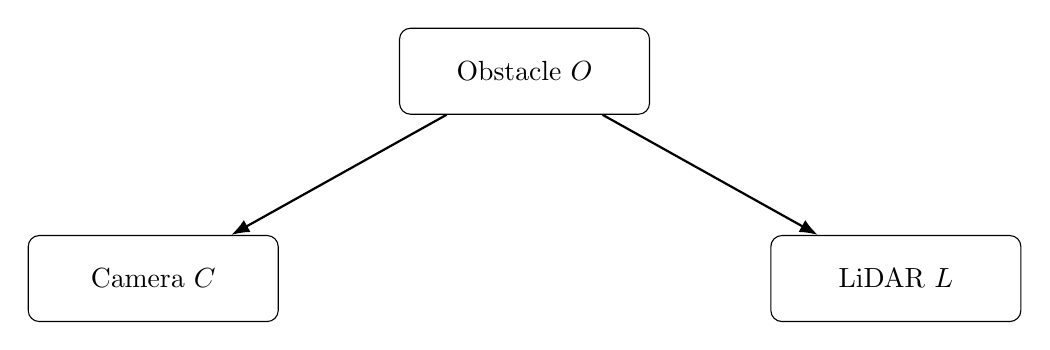
\begin{tikzpicture}[>=Latex,node distance=0.85in,every node/.style={draw,rounded corners,align=center,minimum width=1.25in,minimum height=0.43in}]
    \node (o) {Obstacle $O$};
    \node (c) [below left=of o] {Camera $C$};
    \node (l) [below right=of o] {LiDAR $L$};
    \draw[->,thick] (o)--(c);
    \draw[->,thick] (o)--(l);
  \end{tikzpicture}
  \end{center}

  \begin{keyidea}
    If some unmodeled factor affects both sensors, this factorization double-counts shared evidence.
  \end{keyidea}
\end{frame}

% -----------------------------------------------------------------------------
% Slide 6
% -----------------------------------------------------------------------------
\begin{frame}[shrink=10]{A Shared Cause Breaks the Naive Assumption}
  \begin{center}
  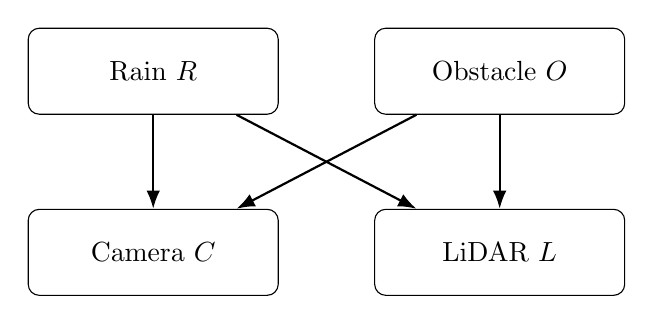
\begin{tikzpicture}[>=Latex,every node/.style={draw,rounded corners,align=center,minimum width=1.25in,minimum height=0.43in}]
    \node (r) at (-2.2,1.2) {Rain $R$};
    \node (o) at ( 2.2,1.2) {Obstacle $O$};
    \node (c) at (-2.2,-1.1) {Camera $C$};
    \node (l) at ( 2.2,-1.1) {LiDAR $L$};
    \draw[->,thick] (r)--(c);
    \draw[->,thick] (r)--(l);
    \draw[->,thick] (o)--(c);
    \draw[->,thick] (o)--(l);
  \end{tikzpicture}
  \end{center}

  Rain is a common cause of sensor errors. If we omit it, $C$ and $L$ can remain correlated even after conditioning on $\neg O$.

  \begin{keyidea}
    The fix is not ``trust the sensors less.'' The fix is to represent the dependency that creates the correlation.
  \end{keyidea}
\end{frame}

% -----------------------------------------------------------------------------
% Slide 7
% -----------------------------------------------------------------------------
\begin{frame}[shrink=10]{Correlated Errors Can Make Us Overconfident}
  Using the model we will build today, when the path is clear:
  \[
    P(C\mid \neg O)=0.09,
    \qquad
    P(L\mid \neg O)=0.056.
  \]

  Naive independence predicts
  \[
    P(C,L\mid \neg O)
    \approx
    0.09(0.056)
    =0.00504.
  \]

  But after accounting for rain,
  \[
    P(C,L\mid \neg O)=0.0108.
  \]

  \begin{keyidea}
    Treating correlated evidence as independent makes repeated agreement look more informative than it really is.
  \end{keyidea}
\end{frame}

\section{Bayesian Network Representation}

% -----------------------------------------------------------------------------
% Slide 8
% -----------------------------------------------------------------------------
\begin{frame}[shrink=10]{Bayesian Networks Make the Structure Explicit}
  \begin{columns}[T,onlytextwidth]
    \begin{column}{0.54\textwidth}
      \begin{cpdefinition}
        A \textbf{Bayesian network} is a directed acyclic graph (DAG) whose nodes are random variables and whose edges define a factorization of their joint probability distribution.
      \end{cpdefinition}

      \begin{itemize}
        \item \textbf{Graph:} which variables directly depend on which others.
        \item \textbf{CPTs:} numerical conditional probabilities at each node.
        \item \textbf{Factorization:} local terms multiply into the joint distribution.
      \end{itemize}
    \end{column}
    \begin{column}{0.40\textwidth}
      \lectureimage[2.75in]{slide8.png}
    \end{column}
  \end{columns}

  \begin{keyidea}
    A Bayes net is both a probability model and a compact statement about conditional independence.
  \end{keyidea}
\end{frame}

% -----------------------------------------------------------------------------
% Slide 9
% -----------------------------------------------------------------------------
\begin{frame}[shrink=10]{Our Robot Network}
  \begin{center}
  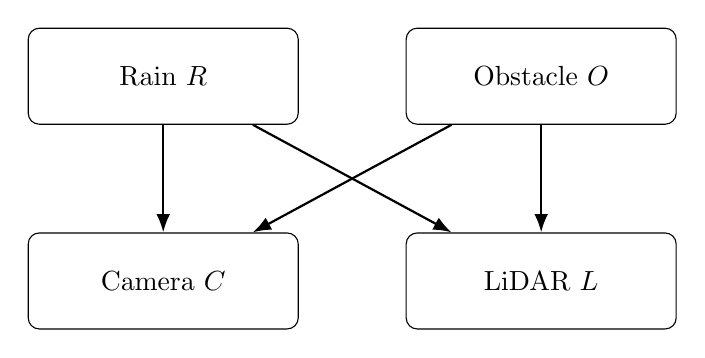
\begin{tikzpicture}[>=Latex,every node/.style={draw,rounded corners,align=center,minimum width=1.35in,minimum height=0.48in}]
    \node (r) at (-2.4,1.3) {Rain $R$};
    \node (o) at ( 2.4,1.3) {Obstacle $O$};
    \node (c) at (-2.4,-1.3) {Camera $C$};
    \node (l) at ( 2.4,-1.3) {LiDAR $L$};
    \draw[->,thick] (r)--(c);
    \draw[->,thick] (r)--(l);
    \draw[->,thick] (o)--(c);
    \draw[->,thick] (o)--(l);
  \end{tikzpicture}
  \end{center}

  The graph says each sensor depends directly on obstacle state and rain---not on every variable in the model.

  \begin{keyidea}
    A sparse graph states which dependencies are worth modeling and which dependencies we are willing to omit.
  \end{keyidea}
\end{frame}

% -----------------------------------------------------------------------------
% Slide 10
% -----------------------------------------------------------------------------
\begin{frame}[shrink=10]{What Does an Arrow Mean?}
  \begin{columns}[T,onlytextwidth]
    \begin{column}{0.47\textwidth}
      \begin{block}{Operational meaning}
        An edge $X\rightarrow Y$ means $Y$'s local probability table is conditioned on $X$.
      \end{block}
    \end{column}
    \begin{column}{0.47\textwidth}
      \begin{block}{Not automatically causation}
        A Bayesian network may have a causal interpretation, but the probabilistic definition only requires a valid DAG and factorization.
      \end{block}
    \end{column}
  \end{columns}

  For the robot,
  \[
    O\rightarrow C
    \quad\Longrightarrow\quad
    P(C\mid O,\ldots),
  \]
  and
  \[
    R\rightarrow C
    \quad\Longrightarrow\quad
    P(C\mid R,\ldots).
  \]

  \begin{keyidea}
    Edges tell us what information the local conditional model needs. Missing edges are equally important.
  \end{keyidea}
\end{frame}

% -----------------------------------------------------------------------------
% Slide 11
% -----------------------------------------------------------------------------
\begin{frame}[shrink=10]{The Graph Factorizes the Joint Distribution}
  For a Bayesian network,
  \[
    P(X_1,\ldots,X_n)
    =
    \prod_i P(X_i\mid Parents(X_i)).
  \]

  For our robot network,
  \[
    P(O,R,C,L)
    =
    P(O)P(R)P(C\mid O,R)P(L\mid O,R).
  \]

  \begin{itemize}
    \item root nodes contribute priors;
    \item each non-root node depends only on its parents;
    \item multiplying the local factors recovers the probability of any complete assignment.
  \end{itemize}

  \begin{keyidea}
    Bayes nets replace one enormous joint table with a product of smaller local tables.
  \end{keyidea}
\end{frame}

% -----------------------------------------------------------------------------
% Slide 12
% -----------------------------------------------------------------------------
\begin{frame}[shrink=10]{Structure Trades Parameters for Assumptions}
  \begin{center}
  \renewcommand{\arraystretch}{1.35}
  \begin{tabular}{l|c|p{0.45\textwidth}}
    \textbf{Representation} & \textbf{Free probabilities} & \textbf{Assumption burden} \\\hline
    Full joint: $O,R,C,L$ & 15 & Almost none \\
    Our Bayes net & 10 & $C\perp\!\!\!\perp L\mid O,R$ \\
    Naive sensor model & 5 & $C\perp\!\!\!\perp L\mid O$ and rain omitted \\
  \end{tabular}
  \end{center}

  Four binary variables have $16$ complete assignments, but a full joint needs only $15$ free values because probabilities must sum to one.

  \begin{keyidea}
    Model structure is compression: we save parameters and computation by declaring which dependencies we believe are unnecessary.
  \end{keyidea}
\end{frame}

\section{Conditional Probability Tables}

% -----------------------------------------------------------------------------
% Slide 13
% -----------------------------------------------------------------------------
\begin{frame}[shrink=10]{Root Nodes Need Priors}
  For today's toy model:

  \begin{columns}[T,onlytextwidth]
    \begin{column}{0.46\textwidth}
      \begin{center}
      \begin{tabular}{c|c}
        \textbf{Obstacle $O$} & \textbf{Probability} \\\hline
        true & 0.10 \\
        false & 0.90
      \end{tabular}
      \end{center}
    \end{column}
    \begin{column}{0.46\textwidth}
      \begin{center}
      \begin{tabular}{c|c}
        \textbf{Rain $R$} & \textbf{Probability} \\\hline
        true & 0.20 \\
        false & 0.80
      \end{tabular}
      \end{center}
    \end{column}
  \end{columns}

  Because these nodes have no parents, their CPTs are simply prior distributions.

  \begin{keyidea}
    A root node still has a CPT---it is just an unconditional probability table.
  \end{keyidea}
\end{frame}

% -----------------------------------------------------------------------------
% Slide 14
% -----------------------------------------------------------------------------
\begin{frame}[shrink=10]{A CPT Encodes the Camera Model}
  \begin{columns}[T,onlytextwidth]
    \begin{column}{0.53\textwidth}
      \begin{center}
      \renewcommand{\arraystretch}{1.25}
      \begin{tabular}{c|c|c}
        \textbf{$O$} & \textbf{$R$} & \textbf{$P(C=+)$} \\\hline
        true & true & 0.85 \\
        true & false & 0.95 \\
        false & true & 0.25 \\
        false & false & 0.05
      \end{tabular}
      \end{center}
    \end{column}
    \begin{column}{0.41\textwidth}
      \begin{block}{Interpret one row}
        $P(C=+\mid O=true,R=true)=0.85$ means rain slightly reduces the camera's true-positive rate.
      \end{block}

      \begin{block}{Interpret another}
        $P(C=+\mid O=false,R=true)=0.25$ means rain also raises the false-positive rate.
      \end{block}
    \end{column}
  \end{columns}

  \begin{keyidea}
    A CPT lets one sensor behave differently under different combinations of its direct parents.
  \end{keyidea}
\end{frame}

% -----------------------------------------------------------------------------
% Slide 15
% -----------------------------------------------------------------------------
\begin{frame}[shrink=10]{The LiDAR Gets Its Own CPT}
  \begin{columns}[T,onlytextwidth]
    \begin{column}{0.53\textwidth}
      \begin{center}
      \renewcommand{\arraystretch}{1.25}
      \begin{tabular}{c|c|c}
        \textbf{$O$} & \textbf{$R$} & \textbf{$P(L=+)$} \\\hline
        true & true & 0.90 \\
        true & false & 0.98 \\
        false & true & 0.20 \\
        false & false & 0.02
      \end{tabular}
      \end{center}
    \end{column}
    \begin{column}{0.41\textwidth}
      \begin{itemize}
        \item LiDAR is more reliable than the camera in this toy model.
        \item Rain still increases its false-positive rate.
        \item Camera and LiDAR can share the effect of rain without directly depending on each other.
      \end{itemize}
    \end{column}
  \end{columns}

  \begin{keyidea}
    Separate local models can still coordinate globally because they share parent variables.
  \end{keyidea}
\end{frame}

% -----------------------------------------------------------------------------
% Slide 16
% -----------------------------------------------------------------------------
\begin{frame}[shrink=10]{CPTs Have Their Own Scaling Problem}
  For a binary child with $k$ binary parents,
  \[
    \text{CPT parent rows}=2^k.
  \]

  \begin{columns}[T,onlytextwidth]
    \begin{column}{0.40\textwidth}
      \begin{center}
      \begin{tabular}{c|r}
        \textbf{Parents} & \textbf{Rows} \\\hline
        2 & 4 \\
        5 & 32 \\
        10 & 1,024 \\
        20 & 1,048,576
      \end{tabular}
      \end{center}
    \end{column}
    \begin{column}{0.52\textwidth}
      \begin{block}{Tradeoff}
        Adding an edge may improve model fidelity, but every extra parent can multiply the number of probabilities we must specify or learn.
      \end{block}
    \end{column}
  \end{columns}

  \begin{keyidea}
    Bayes nets control the full-joint explosion only when each variable has relatively few direct parents.
  \end{keyidea}
\end{frame}

\section{Reading Independence from the Graph}

% -----------------------------------------------------------------------------
% Slide 17
% -----------------------------------------------------------------------------
\begin{frame}[shrink=10]{Conditional Independence Is Now Local and Explicit}
  Our graph asserts
  \[
    C\perp\!\!\!\perp L\mid O,R.
  \]

  In words:
  \begin{block}{What the graph claims}
    If obstacle state and rain are known, then the camera reading provides no additional information about the LiDAR reading, and vice versa.
  \end{block}

  This is a much weaker---and more plausible---assumption than
  \[
    C\perp\!\!\!\perp L\mid O.
  \]

  \begin{keyidea}
    The network does not eliminate independence assumptions; it lets us state the right ones more precisely.
  \end{keyidea}
\end{frame}

% -----------------------------------------------------------------------------
% Slide 18
% -----------------------------------------------------------------------------
\begin{frame}[shrink=10]{The Local Markov Property}
  \begin{cpdefinition}
    Each node in a Bayesian network is conditionally independent of its non-descendants given its parents.
  \end{cpdefinition}

  For the Camera node:
  \begin{itemize}
    \item $Parents(C)=\{O,R\}$;
    \item LiDAR is not a descendant of Camera;
    \item therefore $C\perp\!\!\!\perp L\mid O,R$.
  \end{itemize}

  \begin{keyidea}
    A graph is not just a picture; its topology encodes a family of conditional-independence statements.
  \end{keyidea}
\end{frame}

% -----------------------------------------------------------------------------
% Slide 19
% -----------------------------------------------------------------------------
\begin{frame}[shrink=10]{Pattern 1: A Chain}
  \begin{center}
  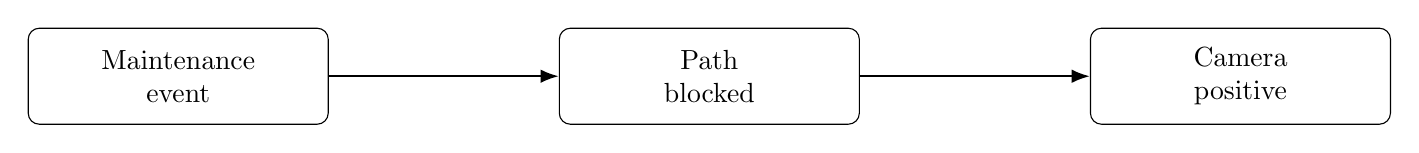
\begin{tikzpicture}[>=Latex,node distance=1.15in,every node/.style={draw,rounded corners,align=center,minimum width=1.5in,minimum height=0.48in}]
    \node (a) {Maintenance\\event};
    \node (b) [right=of a] {Path\\blocked};
    \node (c) [right=of b] {Camera\\positive};
    \draw[->,thick] (a)--(b);
    \draw[->,thick] (b)--(c);
  \end{tikzpicture}
  \end{center}

  \[
    A\rightarrow B\rightarrow C.
  \]

  \begin{block}{Condition on the middle}
    Once $B$ is known, $A$ provides no additional information about $C$.
  \end{block}

  \begin{keyidea}
    In a chain, observing the middle node blocks information flow between the ends.
  \end{keyidea}
\end{frame}

% -----------------------------------------------------------------------------
% Slide 20
% -----------------------------------------------------------------------------
\begin{frame}[shrink=10]{Pattern 2: A Fork / Common Cause}
  \begin{center}
  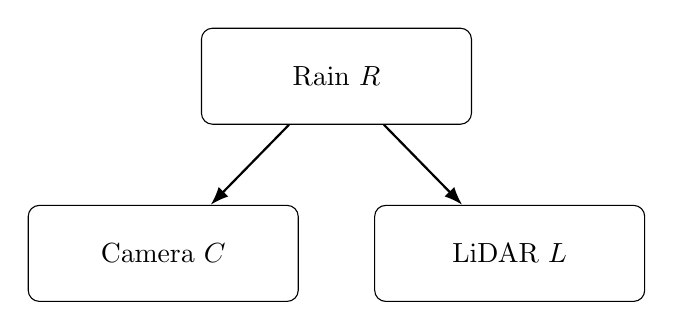
\begin{tikzpicture}[>=Latex,every node/.style={draw,rounded corners,align=center,minimum width=1.35in,minimum height=0.48in}]
    \node (r) at (0,1.25) {Rain $R$};
    \node (c) at (-2.2,-1.0) {Camera $C$};
    \node (l) at ( 2.2,-1.0) {LiDAR $L$};
    \draw[->,thick] (r)--(c);
    \draw[->,thick] (r)--(l);
  \end{tikzpicture}
  \end{center}

  \begin{columns}[T,onlytextwidth]
    \begin{column}{0.47\textwidth}
      \begin{block}{Before observing Rain}
        Camera and LiDAR can be correlated because they share a common cause.
      \end{block}
    \end{column}
    \begin{column}{0.47\textwidth}
      \begin{block}{After observing Rain}
        Conditioning on the common cause can block that dependence.
      \end{block}
    \end{column}
  \end{columns}
\end{frame}

% -----------------------------------------------------------------------------
% Slide 21
% -----------------------------------------------------------------------------
\begin{frame}[shrink=10]{Pattern 3: A Collider}
  \begin{center}
  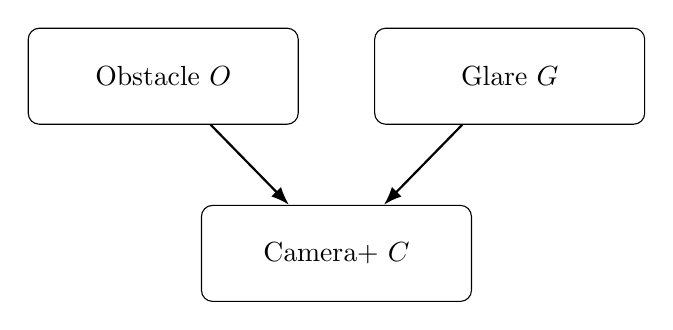
\begin{tikzpicture}[>=Latex,every node/.style={draw,rounded corners,align=center,minimum width=1.35in,minimum height=0.48in}]
    \node (o) at (-2.2,1.25) {Obstacle $O$};
    \node (g) at ( 2.2,1.25) {Glare $G$};
    \node (c) at (0,-1.0) {Camera+ $C$};
    \draw[->,thick] (o)--(c);
    \draw[->,thick] (g)--(c);
  \end{tikzpicture}
  \end{center}

  \begin{block}{Counterintuitive rule}
    The two causes can be independent before observing $C$, but become dependent after we condition on their common effect.
  \end{block}

  \begin{keyidea}
    Colliders behave opposite to chains and forks: conditioning can open a dependency instead of blocking it.
  \end{keyidea}
\end{frame}

% -----------------------------------------------------------------------------
% Slide 22
% -----------------------------------------------------------------------------
\begin{frame}[shrink=10]{Explaining Away}
  Suppose the camera fires. Two explanations are plausible:
  \begin{itemize}
    \item there really is an obstacle;
    \item sun glare caused a false positive.
  \end{itemize}

  Now LiDAR also fires.

  \begin{block}{Posterior effect}
    LiDAR evidence makes ``obstacle'' more plausible, so the camera reading needs ``glare'' less as an explanation.
  \end{block}

  \begin{center}
  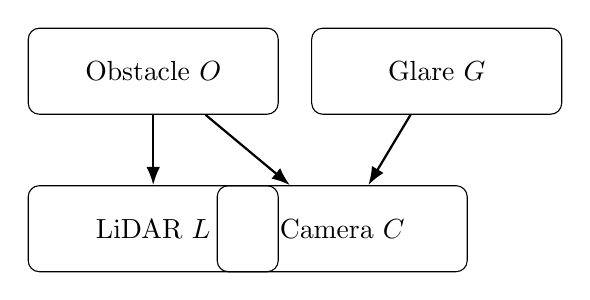
\begin{tikzpicture}[>=Latex,every node/.style={draw,rounded corners,align=center,minimum width=1.25in,minimum height=0.43in}]
    \node (o) at (-1.8,1.0) {Obstacle $O$};
    \node (g) at ( 1.8,1.0) {Glare $G$};
    \node (l) at (-1.8,-1.0) {LiDAR $L$};
    \node (c) at ( 0.6,-1.0) {Camera $C$};
    \draw[->,thick] (o)--(l);
    \draw[->,thick] (o)--(c);
    \draw[->,thick] (g)--(c);
  \end{tikzpicture}
  \end{center}

  \begin{keyidea}
    Conditioning can create dependence as well as remove it. Colliders are the key exception.
  \end{keyidea}
\end{frame}

% -----------------------------------------------------------------------------
% Slide 23
% -----------------------------------------------------------------------------
\begin{frame}[shrink=10]{d-Separation: A Compact Independence Test}
  \begin{center}
  \renewcommand{\arraystretch}{1.30}
  \begin{tabular}{l|c|l}
    \textbf{Path pattern} & \textbf{Condition on middle?} & \textbf{Effect} \\\hline
    $A\rightarrow B\rightarrow C$ & yes & blocks path \\
    $A\leftarrow B\rightarrow C$ & yes & blocks path \\
    $A\rightarrow B\leftarrow C$ & no & path blocked by default \\
    $A\rightarrow B\leftarrow C$ & yes, on $B$ or descendant & opens path \\
  \end{tabular}
  \end{center}

  \begin{cpdefinition}
    Two variables are d-separated by the evidence when every path between them is blocked under these rules.
  \end{cpdefinition}

  \begin{keyidea}
    The graph lets us answer many independence questions without multiplying a single probability.
  \end{keyidea}
\end{frame}

\section{Exact Inference}

% -----------------------------------------------------------------------------
% Slide 24
% -----------------------------------------------------------------------------
\begin{frame}[shrink=10]{Inference Means Asking the Network a Query}
  We want
  \[
    P(O\mid C=+,L=+).
  \]

  \begin{columns}[T,onlytextwidth]
    \begin{column}{0.30\textwidth}
      \begin{block}{Query variable}
        $O$: Is there actually an obstacle?
      \end{block}
    \end{column}
    \begin{column}{0.30\textwidth}
      \begin{block}{Evidence}
        $C=+,L=+$: both sensors fired.
      \end{block}
    \end{column}
    \begin{column}{0.30\textwidth}
      \begin{block}{Hidden variable}
        $R$: rain is not directly observed in this query.
      \end{block}
    \end{column}
  \end{columns}

  Exact inference sums over every hidden state consistent with the evidence.

  \begin{keyidea}
    A Bayes-net query is probability calculation under the factorization encoded by the graph.
  \end{keyidea}
\end{frame}

% -----------------------------------------------------------------------------
% Slide 25
% -----------------------------------------------------------------------------
\begin{frame}[shrink=10]{Exact Inference by Enumeration}
  Because Rain is hidden, sum over both rain states:
  \[
    P(O\mid c,l)
    =
    \alpha
    \sum_r
    P(O)P(r)P(c\mid O,r)P(l\mid O,r).
  \]

  The normalization constant $\alpha$ makes the two obstacle states sum to one.

  \begin{block}{Enumeration}
    Instantiate hidden variables, compute the joint probability for each assignment, sum the compatible assignments, then normalize.
  \end{block}

  \begin{keyidea}
    The BN factorization tells us exactly which local CPT entries to multiply for each hidden assignment.
  \end{keyidea}
\end{frame}

% -----------------------------------------------------------------------------
% Slide 26
% -----------------------------------------------------------------------------
\begin{frame}[shrink=10]{Worked Query: Score the Obstacle Hypothesis}
  \[
    P(O,c,l)
    =
    P(O)\sum_r P(r)P(c\mid O,r)P(l\mid O,r).
  \]

  Rain branch:
  \[
    (0.20)(0.85)(0.90)=0.153.
  \]

  No-rain branch:
  \[
    (0.80)(0.95)(0.98)=0.7448.
  \]

  Therefore
  \[
    P(O,c,l)
    =
    0.10(0.153+0.7448)
    =0.08978.
  \]

  \begin{keyidea}
    Hidden variables are not ignored; exact inference marginalizes over them.
  \end{keyidea}
\end{frame}

% -----------------------------------------------------------------------------
% Slide 27
% -----------------------------------------------------------------------------
\begin{frame}[shrink=10]{Score the Clear Hypothesis, Then Normalize}
  \[
    P(\neg O,c,l)
    =
    0.90\Big[(0.20)(0.25)(0.20)+(0.80)(0.05)(0.02)\Big]
    =0.00972.
  \]

  Normalize:
  \[
    P(O\mid c,l)
    =
    \frac{0.08978}{0.08978+0.00972}
    \approx 0.902.
  \]

  \begin{columns}[T,onlytextwidth]
    \begin{column}{0.47\textwidth}
      \begin{block}{Structured posterior}
        About $90.2\%$: rain can jointly explain two positive sensor readings.
      \end{block}
    \end{column}
    \begin{column}{0.47\textwidth}
      \begin{block}{Naive posterior}
        About $95.2\%$ if the correlated evidence is incorrectly multiplied as independent.
      \end{block}
    \end{column}
  \end{columns}

  \begin{keyidea}
    The difference is not a new Bayes rule; it comes from a better factorization of the evidence-generating process.
  \end{keyidea}
\end{frame}

% -----------------------------------------------------------------------------
% Slide 28
% -----------------------------------------------------------------------------
\begin{frame}[shrink=10]{Variable Elimination Reuses the Factorization}
  Enumeration is correct, but larger networks repeatedly multiply the same subexpressions.

  Eliminate Rain into a temporary factor:
  \[
    f(O)
    =
    \sum_r P(r)P(c\mid O,r)P(l\mid O,r).
  \]

  Then finish with
  \[
    P(O\mid c,l)=\alpha P(O)f(O).
  \]

  \begin{cpdefinition}
    \textbf{Variable elimination} is an exact inference algorithm that multiplies relevant factors and sums out hidden variables in an organized order.
  \end{cpdefinition}

  \begin{keyidea}
    Same probability calculation, less repeated work. On larger networks, elimination order can determine whether inference is practical.
  \end{keyidea}
\end{frame}

\section{Tradeoffs and Synthesis}

% -----------------------------------------------------------------------------
% Slide 29
% -----------------------------------------------------------------------------
\begin{frame}[shrink=10]{Exact Does Not Mean Cheap}
  \begin{columns}[T,onlytextwidth]
    \begin{column}{0.54\textwidth}
      \begin{itemize}
        \item Sparse graphs can make local CPTs small and inference efficient.
        \item Dense dependencies create large CPTs and large intermediate factors.
        \item Variable elimination can still be exponential in the network's induced width / treewidth.
        \item Choosing or learning the graph structure is itself a modeling problem.
      \end{itemize}
    \end{column}
    \begin{column}{0.40\textwidth}
      \lectureimage[2.75in]{slide29.png}
    \end{column}
  \end{columns}

  \begin{keyidea}
    Bayesian networks trade unrestricted dependence for structured dependence. Good structure can buy tractability; dense structure can lose it.
  \end{keyidea}
\end{frame}

% -----------------------------------------------------------------------------
% Slide 30
% -----------------------------------------------------------------------------
\begin{frame}[shrink=10]{Takeaways}
  \begin{itemize}
    \item Naive Bayes is useful because of a strong conditional-independence assumption.
    \item Shared causes can correlate sensors and make naive evidence multiplication overconfident.
    \item A Bayesian network is a DAG plus local conditional probability tables.
    \item Its graph factorizes the joint distribution and encodes conditional independences.
    \item Chains, forks, and colliders behave differently under conditioning.
    \item Exact inference marginalizes hidden variables; variable elimination organizes that computation.
    \item The central tradeoff is model fidelity versus parameter count and computational cost.
  \end{itemize}

  \begin{keyidea}
    Today: represent structured uncertainty exactly. Next: what happens when exact inference itself becomes too expensive?
  \end{keyidea}
\end{frame}

\end{document}
